% siminos/talks/DDaysE12/DDaysE12.tex      pdflatex DDaysE12
% $Author: predrag $
% $Date: 2012-08-08 16:16:55 +0200 (Wed, 08 Aug 2012) $


% Evangelos Dynamics Days Europe 2012 talk  2012.09.06
% used as template:
% Predrag GT math colloquium                2012.03.26
% derived from
% talks/predrag/continuous/continuous.tex   2011.09.09
% Predrag beamer format                     2011.06.17
% Predrag                                   2011.04.12
% derived from
% siminos/talks/Dresden10/symmReduc.tex 	2010.06.29
% Predrag Eckmann's haeberli slide style    2005.05.03
%    ChaosBook/version 11 slides
%	 from ChaosBook continuous.tex

% might want to use text from
%    predrag/lectures/Goth11/Cphg11abstr.txt
%    predrag/lectures/maribor/11/abscvitancourse.tex

\input ../../inputs/layoutBeamerES
\input ../../inputs/def % no edits, always from dasbuch/book/inputs
\input ../../inputs/defsBeamer
                          \date{{\scriptsize
Dynamics Days Europe\\
 6 September 2012
                          }}

\title{Continuous symmetry reduction\\ in high-dimensional flows
with the method of slices
     }
\author{\underline{Evangelos Siminos}\\
    Max Planck Inst. for the Physics of Complex Systems\vspace{20pt}\\
    Predrag~Cvitanovi\'c \\
    Georgia Tech
}


\begin{document}

\section{Symmetries}

\begin{frame}{}
  \titlepage
\end{frame}

\begin{frame}{Motivation}
 \begin{center}
  \includegraphics[width=0.3\textwidth,clip=true] %,height=0.5\textheight
  {CLEx1x2z}
  ~~~~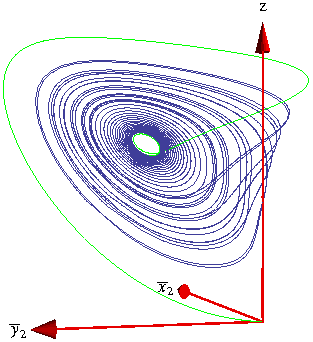
\includegraphics[width=0.3\textwidth,clip=true]
  {CLEinvXYZ}
\end{center}
 \begin{itemize}
  \item Continuous symmetry induces drifts
  \item Transform to equivalent attractor (no loss of information)
  \item ODEs (Complex Lorenz equations)
  \item PDEs (Kuramoto-Sivashinsky equation)
 \end{itemize}

\end{frame}

\begin{frame}{symmetry of a dynamical system}

\begin{block}{\statesp}
a manifold $\pS \in \reals^{d}$ :
$d$ numbers determine the state of the system
\end{block}

\bigskip

\begin{block}{representative point }
$\ssp(t) \in \pS$
\\
a state of physical system at instant in time
\end{block}


\begin{block}{deterministic dynamics}
map $\timeflow(\xInit)$ =
representative point time $t$ later
\end{block}
\begin{block}{a group $\Group$ is a {symmetry} of the dynamics if}
for every solution $f^t(\ssp) \in \pS$ and  $\LieEl \in \Group$,
$\LieEl f^t(\ssp)$ is also a solution
\end{block}
\end{frame}


\begin{frame}{Complex Lorenz equations (CLE)}
  \begin{exampleblock}{}
	\begin{align*}
	  \dot{x} &= -\sigma x+ \sigma y \,,\continue
	  \dot{y} &=\, (\rLor-z)x-a y\,, \continue
	  \dot{z} &= (x y^*+x^*y)/2 -b z\,.
	\end{align*}
  \end{exampleblock}
  \begin{block}{}
     \begin{itemize}
	  \item $x,y\in\Clx{}$, $z\in\Rls{}$
	  \item $\sigma,\,b \in \Rls{}$, $\rLor=\RerCLor+i\ImrCLor$, $a=1-i e$
	  \end{itemize}
  \end{block}
\end{frame}


\begin{frame}{\SOn{2} invariance}
			\begin{exampleblock}{{\cLe}}
\scriptsize		
\[
		\left[
					\begin{array}{c}
				\dot{x}_1 \\ \dot{x}_2 \\ \dot{y}_1 \\ \dot{y}_2 \\ \dot{z}
				\end{array}
		\right]
=
		\left[
					\begin{array}{c}
				 -\sigma x_1 + \sigma y_1 \\
				-\sigma x_2 + \sigma y_2 \\
                (\RerCLor-z) x_1 - \ImrCLor x_2 -y_1-e y_2 \\
                \ImrCLor x_1 + (\RerCLor-z) x_2 + e y_1- y_2 \\
				-b z + x_1 y_1 + x_2 y_2
				\end{array}
		\right]
\]
$x=x_1+i\,x_2$, $y=y_1+i\,y_2$.
			\end{exampleblock}

\begin{block}{}
invariant under a \SOn{2} rotation by finite angle
\gSpace:
\scriptsize		
\[
\LieEl(\gSpace) \,=\,  \left(\barr{ccccc}
  \cos \gSpace  & \sin \gSpace  & 0 & 0 & 0 \\
 -\sin \gSpace  & \cos \gSpace  & 0 & 0 & 0 \\
 0 & 0 &  \cos \gSpace & \sin \gSpace   & 0 \\
 0 & 0 & -\sin \gSpace & \cos \gSpace   & 0 \\
 0 & 0 & 0             & 0              & 1
    \earr\right)
\] %{CLfRots}
\end{block}
%\begin{block}{\statesp\ decomposition}
%\begin{enumerate}
%  \item $m=0$ \SOn{2}-invariant subspace: $z$-axis
%  \item $m=1$ subspace with multiplicity 2
%\end{enumerate}
%\end{block}
\end{frame}


\begin{frame}{CLE phase space}
 \begin{block}{continuous symmetry induces drifts}
\begin{center}
  \includegraphics[width=0.35\textwidth,clip=true] %,height=0.5\textheight
  {CLEchaotic}
  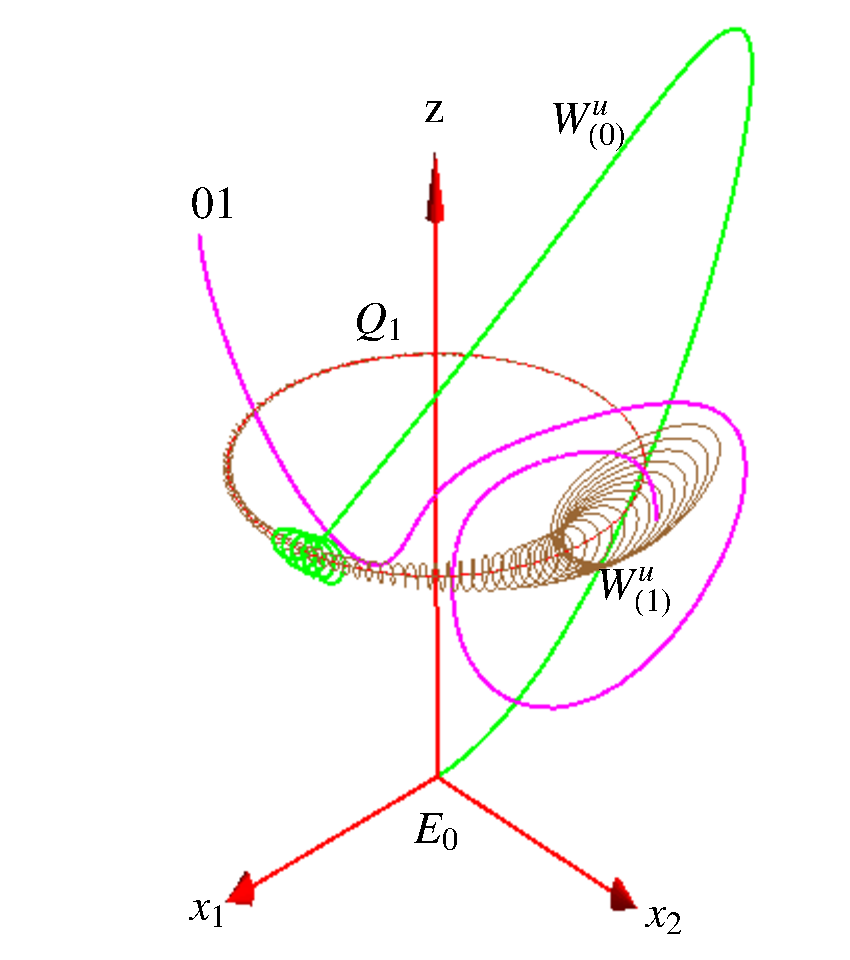
\includegraphics[width=0.35\textwidth,clip=true]
  {CLEcompact}
\end{center}
\end{block}
\begin{itemize}
  \item generic chaotic trajectory (blue)
  \item $E_0$ \eqv  %\EQV{0}
  \item $E_0$ unstable manifold - a cone of such (green)
  \item $Q_1$ \reqv\ (red)
  \item $Q_1$ unstable manifold, one for each point on $Q_1$ (brown)
  \item \rpo\ \cycle{01}, $x(T)=\LieEl(\gSpace)x(0)$ (purple)
\end{itemize}
\end{frame}

\begin{frame}{trajectories, orbits}
%  \caption{\label{fig:A27wurst}
	\begin{columns}[t]
	\column{.32\textwidth}
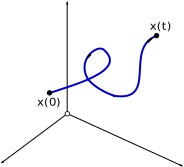
\includegraphics[width=0.95\textwidth]{A27traj}

trajectory $\ssp(\zeit)$
	\column{.32\textwidth}
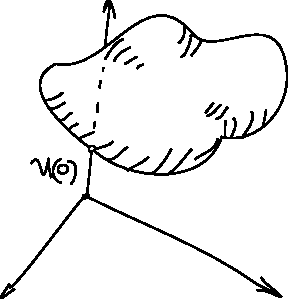
\includegraphics[width=0.95\textwidth]{A27gOrbit}

group orbit $\LieEl\,\ssp(0)$
	\column{.32\textwidth}
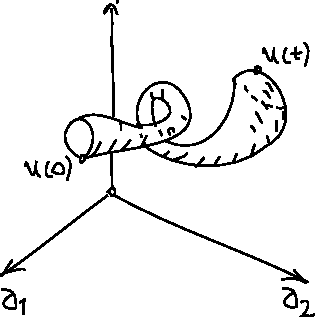
\includegraphics[width=0.95\textwidth]{A27wurst}

wurst $\LieEl\,\ssp(\zeit)$
	\end{columns}
\end{frame}

\begin{frame}{Group orbits}
  \begin{columns}
  \column{0.5\textwidth}
\begin{block}{}
% 2011-08-23 Predrag: previously BeThTraj.pdf from
% dasbuch/book/FigSrc/inkscape/BeThTraj.svg
%  2011-09-09 Predrag: updated continuous.tex overheads
%  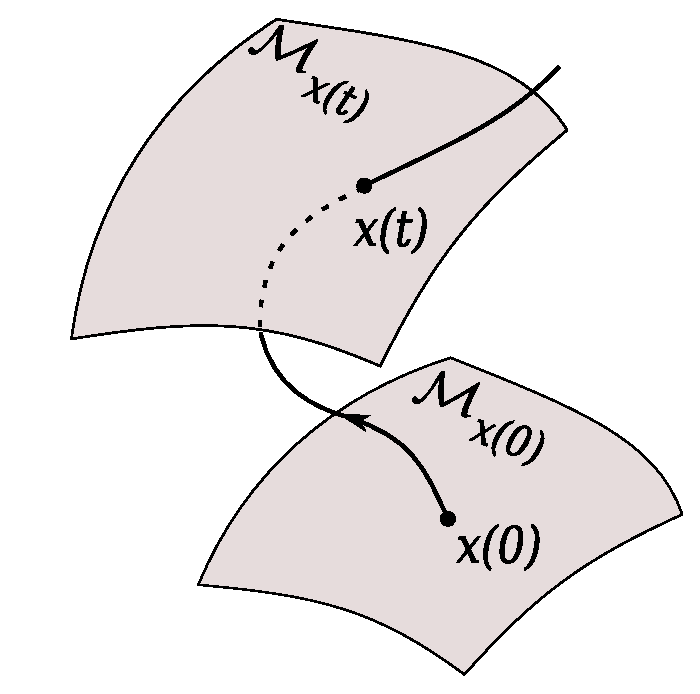
\includegraphics[width=1.00\textwidth,clip=true]{BeThTraj}
 \begin{center}
  \setlength{\unitlength}{1.00\textwidth}
  %% \unitlength = units used in the Picture Environment
  \begin{picture}(1,1.07471658)%
    \put(0,0){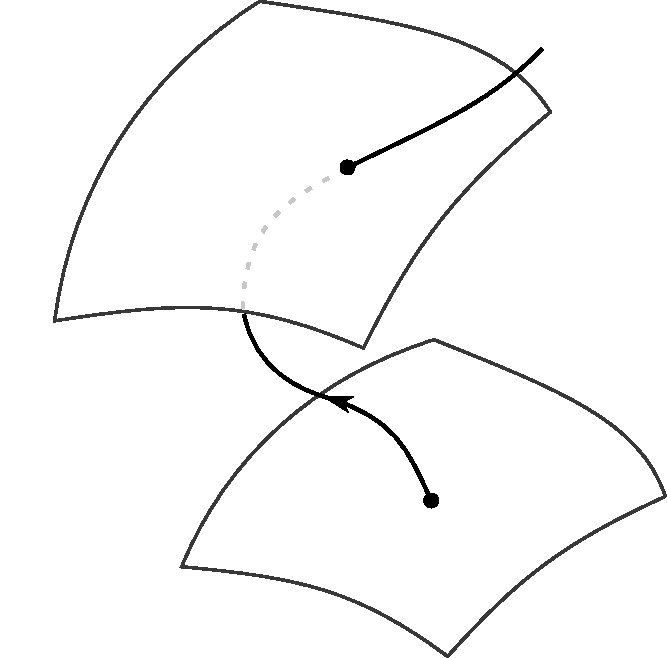
\includegraphics[width=\unitlength]{BeThTrajTeX}}%
    \put(0.28879298,1.02196543){\color[rgb]{0,0,0}\rotatebox{-22.37140782}{\makebox(0,0)[lb]{\smash{$\pS_{\ssp(\tau)}$}}}}%
    \put(0.55566402,0.45078735){\color[rgb]{0,0,0}\rotatebox{-16.6673442}{\makebox(0,0)[lb]{\smash{$\pS_{\ssp(0)}$}}}}%
    \put(0.63028127,0.18433597){\color[rgb]{0,0,0}\rotatebox{0.03136739}{\makebox(0,0)[lb]{\smash{$\ssp(0)$}}}}%
    \put(0.46253394,0.70182304){\color[rgb]{0,0,0}\rotatebox{0.03136739}{\makebox(0,0)[lb]{\smash{$\ssp(\tau)$}}}}%
    \put(0.03852492,0.09250899){\color[rgb]{0,0,0}\rotatebox{0.11031334}{\makebox(0,0)[lb]{\smash{$\pS$}}}}%
  \end{picture}%
 \end{center}
\end{block}
  \column{0.5\textwidth}
\noindent
\emph{group orbit} $\pS_\ssp $ of $\ssp$ is the set of all points visited under the 
action of the group on $\ssp$
\[
\pS_\ssp = \{\LieEl\,\ssp \mid \LieEl \in {\Group}\}
\]
\noindent
any point on the manifold $\pS_{\ssp}$ is
equivalent to any other

\end{columns}
\end{frame}

\section{symmetry reduction}

\begin{frame}{}
\begin{block}{the goal}
replace each group orbit by a unique
point in a lower-dimensional

\bigskip

\hfill
\textcolor{red}{\Large symmetry \reducedsp\ $\pS/\Group$}
\end{block}
\end{frame}

\begin{frame}{symmetry reduction}
  \begin{columns}
  \column{0.5\textwidth}
\begin{block}{full \statesp}
 \begin{center}
  \setlength{\unitlength}{1.00\textwidth}
  %% \unitlength = units used in the Picture Environment
  \begin{picture}(1,1.07315413)%
    \put(0,0){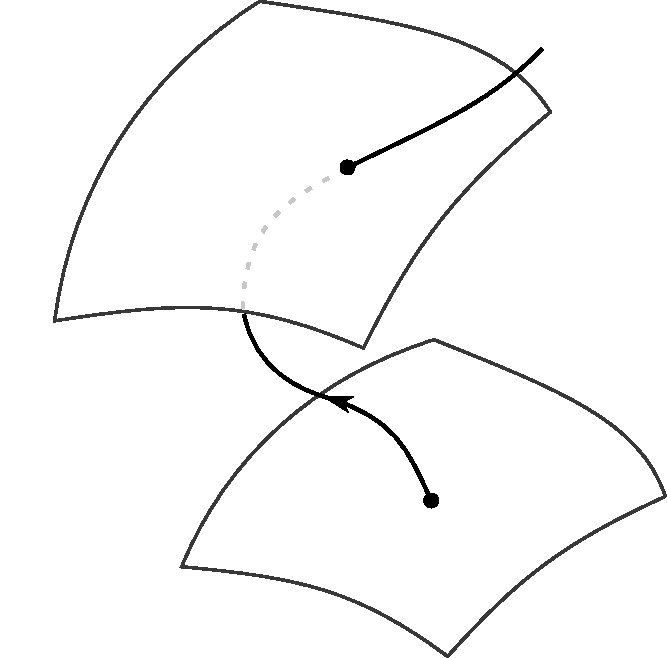
\includegraphics[width=\unitlength]{BeThTrajTeX}}%
    \put(0.30362031,0.99939308){\color[rgb]{0,0,0}\rotatebox{-31.32889204}{\makebox(0,0)[lb]{\smash{$\pS_{\ssp(\tau)}$}}}}%
    \put(0.5686188,0.45975596){\color[rgb]{0,0,0}\rotatebox{-40.8073288}{\makebox(0,0)[lb]{\smash{$\pS_{\ssp(0)}$}}}}%
    \put(0.63028127,0.18433598){\color[rgb]{0,0,0}\rotatebox{0.03136739}{\makebox(0,0)[lb]{\smash{$\ssp(0)$}}}}%
    \put(0.46253394,0.70182305){\color[rgb]{0,0,0}\rotatebox{0.03136739}{\makebox(0,0)[lb]{\smash{$\ssp(\tau)$}}}}%
  \end{picture}%
 \end{center}
\end{block}
  \column{0.5\textwidth}
\begin{block}{\reducedsp}
 \begin{center}
  \setlength{\unitlength}{1.00\textwidth}
  %% \unitlength = units used in the Picture Environment
  \begin{picture}(1,1.07315413)%
    \put(0,0){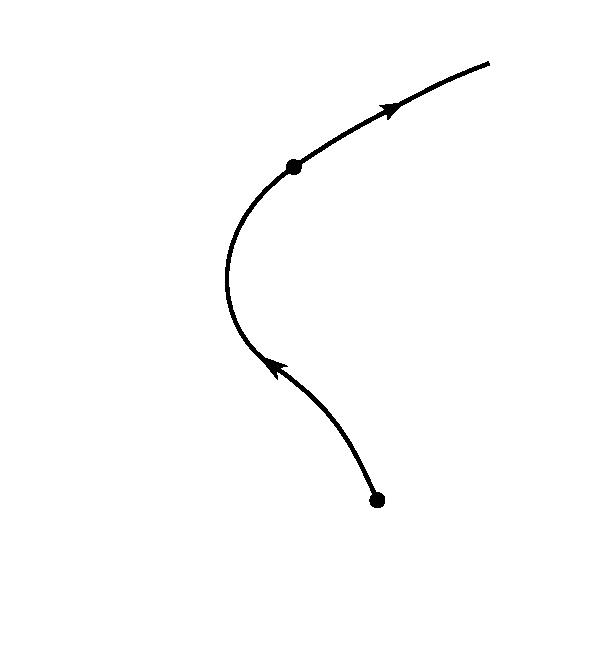
\includegraphics[width=\unitlength]{BeThRedTeX}}%
    \put(0.19912369,0.17144733){\color[rgb]{0,0,0}\rotatebox{0.11031334}{\makebox(0,0)[lb]{\smash{$\pSRed$}}}}%
    \put(0.63028127,0.18433598){\color[rgb]{0,0,0}\rotatebox{0.03136739}{\makebox(0,0)[lb]{\smash{$\sspRed(0)$}}}}%
    \put(0.46253394,0.70182305){\color[rgb]{0,0,0}\rotatebox{0.03136739}{\makebox(0,0)[lb]{\smash{$\sspRed(\tau)$}}}}%
  \end{picture}%
 \end{center}
\end{block}
\end{columns}
\end{frame}

\begin{frame}{The method of slices}
 \begin{block}{}
  \begin{columns}
	\column{0.5\textwidth}
	  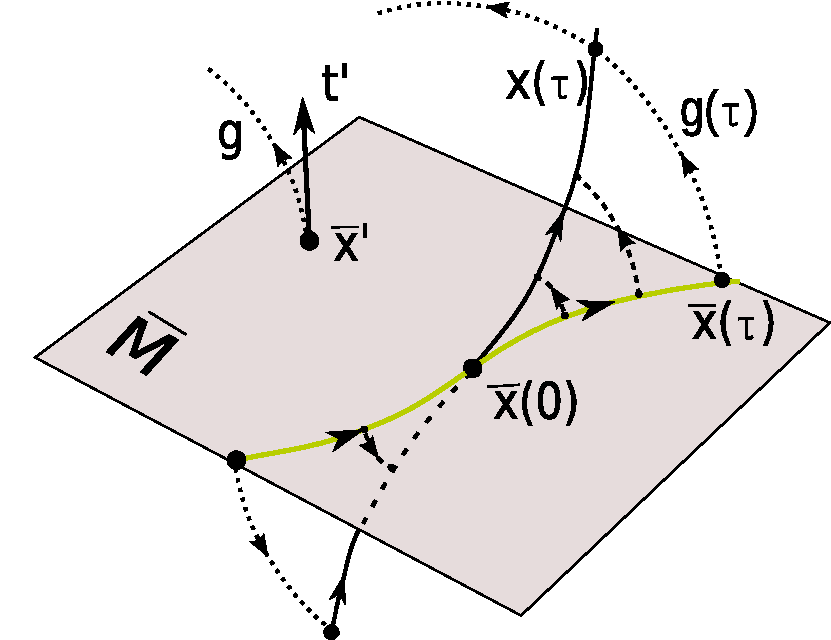
\includegraphics[width=\textwidth]{ReducTraj3.pdf}
	\column{0.5\textwidth}
	\begin{itemize}
	  \item Pick a 'template' $\overline{x}'$.
	  \item Define a slice hyperplane $\overline{M}$ transverse to the group tangent at $\overline{x}'$.
	  \item Find point $\overline{\ssp}(\tau)$ in group orbit of $\ssp(\tau)$ which intersects $\overline{M}$.
	\end{itemize}

  \end{columns}
 \end{block}

\end{frame}

\begin{frame}{Application in CLe}
 
\end{frame}

\section{PDEs}

\begin{frame}{Kuramoto-Sivashinsky equation (KSe)}
 
\end{frame}

\begin{frame}{Symmetries of KSe}
 
\end{frame}

\begin{frame}{Solutions of KSe}
 
\end{frame}

\begin{frame}{40000 relative periodic orbits}
 how are they organized?
\end{frame}

\begin{frame}{Relative periodic orbits on a slice}
 
\end{frame}

\begin{frame}{Poincar\'e Section}
 
(No return map) Unstable manifold of shortest orbit organizes the longer orbits

\end{frame}

\begin{frame}{Conclusions and work in progress}
 
 
\end{frame}




\end{document}
